\documentclass{Rpd}


\begin{document}

\def\Sectitle{Section Title}%%This line can be removed if there is no
						%%section title

\def\copyrightyear{2004}%

\title[short Title]{Measuring Regener-Pfotzer maximum using different types of ionizing radiation detectors and a new telemetry system}
\author[Sample \textit{et~al}]{Author\,$^{\rm a}$, Author\,$^{\rm b}$\footnote{to whom correspondence should be addressed}}
\address{$^{\rm a}$Address followed, $^{\rm b}$Address followed}

\date{Received on April 2, 2003, revised on November 19, 2003,
  accepted on December 22, 2003}

\begin{abstract}
Regener-Pfotzer maximum is located at the altitude where the intensity of cosmic radiation is greatest, usually around 20 km. However, its exact location depends on many parameters such as atmospheric conditions, geographical locations, solar activity and also the type of detected particles. During experimental flights of stratospheric balloons we use different types of ionizing radiation detectors: Geiger-Muller tubes, SPACEDOS silicon detectors and AIRDOS-C scintillation detectors with NaI(Tl) crystal.

Due to necessary data processing of data measured by instruments, the balloon gondolaradiation measurements carriescarry a number of additional supplementary sensors measuring humidity, temperature, location and orientation, altitude, atmospheric pressure, acceleration, etc. All of these sensors have to be monitored during the launch of the stratospheric balloon in order to verify their correct function and furthermore, it is necessary to record their data during the flight for future processing. This was the reason why a new universal system TF-ATMON was gradually developed during the flights of FIK-5 to FIK-6 that is able to solve the above mentioned problems. The system is based on using already existing tools of the PX4 open-source project that makes it possible, apart from data recording and monitoring, to solve other related issues - the possibility to trace the balloon gondola after the flight. For this reason, the originally used telemetry system was made significantly more robust and an IoT LoRa transmitter was added to the system, making it possible to transmit the data necessary for tracing the gondola to the TheThingsNetwork. In this way, a high reliability of finding the gondola and recording the data is ensured. In case of active detectors, it is also necessary that the flight trajectory is recorded synchronously with the supplementary quantities.
The proposed TF-ATMON system is very variable and thus it can be used in other applications than just balloon measurements. However, its application will be demonstrated on stratospheric balloon flights measuring parameters of Regener-Pfotzer maximum.

\end{abstract}

\maketitle


\section{Introduction}

Particles of primary cosmic radiation with sufficient energy interact in the upper part of the atmosphere and generate showers of secondary cosmic radiation. With increasing depth of the atmosphere the intensity of primary radiation decreases whereas the secondary component increases. At an altitude of about 20 km the intensity of secondary cosmic radiation reaches its maximum, called the Pfotzer maximum [Pfotzer, 1936; Regener, 1933; Regener and Pfotzer, 1935]. The Pfotzer maximum varies with geomagnetic vertical cutoff rigidity and with solar cycle and it is generally located at 15-27 km [Bazilevskaya and Svirzhevskaya, 1998]. 
In the past, several experiments were done with the aim to measure vertical profile of ionization in the atmosphere at various locations in the word, mainly using radiosondes consistinged of Geiger tubes [Bazilevskaya and Svirzhevskaya, 1998; Yaniv et al., 2016; Harrison et al., 2014; Sarkar et al., 2017; Li et al., 2007;...], or to characterize instruments? response used for space-based missions [Lawrence et al., 2018; Mukherjee et al., 2016; Urbar et al., 2011; ...]. 
To investigate cosmic radiation at high altitudes (around and above Regener-Pfotzer maximum region) and to test new detectors for cosmic radiation measurements, stratospheric balloons are very useful. 
However, the radiation measurement instruments need to be supplemented also by other sensors measuring temperature, pressure, humidity, altitude, acceleration, etc.  All these sensors should be continuously monitored during the launch and the flight of the balloon to verify their proper function and theirthe values have to be recorded for further processing of all obtained data. 
Platform developed for experiments at different altitudes consisting of a balloon tracking system and different measuring instruments will be presented. The universal system TF-ATMON, based on the use of existing tools of the open-source project PX4 and supplemented with an IoT LoRa transmitter, enables it to monitor and record data during the flight and to trace the balloon. The application is demonstrated on stratospheric balloon flight FIK-6. Various radiation detectors - Geiger-Mueller tubes, Si-diode based detector SPACEDOSSpacedos, and scintillation detectors AIRDOSAirdos-C with inorganic scintillation crystals - were used to measure the vertical profile of cosmic radiation in the atmosphere. 



\section{Materials and methods}

During the first measurements, the construction of balloon gondola was always designed for the use of specific detectors. Balloon avionics was therefore built around the chosen detectors.
This concept led to a situation when every new flight meant a significant amount of work despite the fact that a number of components was recycled every year and used the next one. The reason was the need to adapt the avionics to the innovated version of detectors.

Due to a relatively high value of payload it was necessary to ensure the return of the gondola every flight. The main construction criteria were as follows:

\begin{itemize}
\item Reliable transmission of information about the geographical location of the gondola 
\item Good resistance to impact
\item Ensuring the function in freezing conditions
\end{itemize}

Due to the fact that since the first flight there were various partial shortcomings and despite the generally successful nature of all fights and the fact that the gondola was always found, we tried different technologies to eliminate the complications, which have emerged. During the last experimental flights these included the way the data is recorded.
 
An overall overview of the success of the used technologies is summarized in the following table, with colours representing a degree of reliability:
 


Apart from technologies used in gondolas a number of supplementary tools have undergone intensive development. For example, in order to find the balloon it was necessary to have an accurate real-time map of its position together with a prediction of the subsequent flight and the site of impact. In the case of the last two flights, FIK-5 and FIK-6, the problem is solved by tracker.habhub.org .
As can be seen from the table, during the last flights the avionics was implemented using an UAV technology. It uses the Pixhawk autopilot with PX4 firmware. Telemetry is implemented by a very reliable combination of LoRa modem and SiK modem. Power is provided by Li-ion 18650 batteries that also have a reliable flight history.


\subsection{Universal avionics}

Based on our experience we have used a universal concept of avionics called TF-ATMON that makes it possible to connect different types of payloads and carry out various atmospheric measurements. Furthermore, it provides the detectors with basic services such as power supply, time and position information and provides a possibility to record data in a common log. Therefore it is extremely useful for testing high-altitude cosmic radiation detectors and dosimeters.

%\begin{center}
%\begin{figure*}%avionic
%	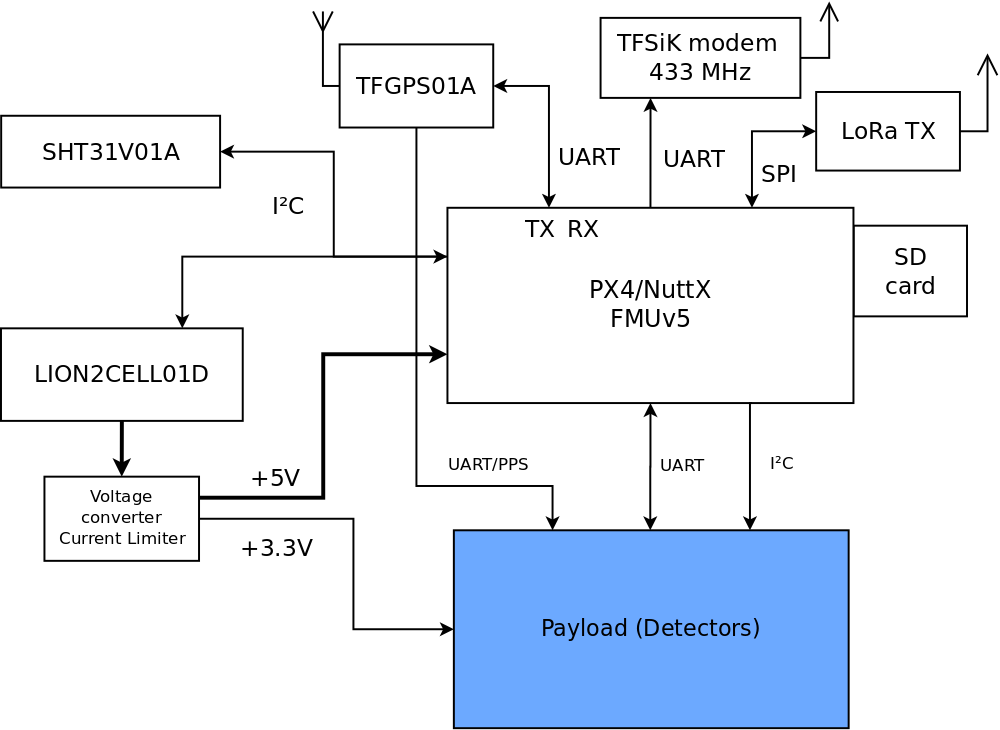
\includegraphics[width=150mm]{avionics_block_schematics.png}
%	\caption{The schematic diagram of the new avionics}
%\end{figure*}
%\end{center}

Transition to the concept, where the balloon specific parts of avionics are completely separate from the system of detectors, simplified the realization of next balloon flights. It reduced the complexity of connecting different types of detectors and at the same time it improved the integrity of supplementary data measurements. Overall, the new features can be summarized by the following.

\begin{itemize}
\item Easy implementation of different payloads
\item Redundant telemetry link
\item Gondola orientation tracking and logging
\item Reliable IMU sensor processing and calibration
\item Possible use of relative high-power payloads
\item Pre-flight continuous charging as an option
\item Power monitoring and maximum uptime calculation relevant to actual temperature
\end{itemize}


\subsection{Further improvements}


As can be seen from the table, the last unsolved problem with the balloon flights is the landing site. Therefore, in the future flights we are planning to use the autopilot for a controlled descent as well.
The descent will be carried out using an unmanned autogyro carrying a payload. The purpose of this solution is in using the autogyro?s rotor instead of the original parachute as it has the advantage of good controllability. Thus it would be possible to choose the landing site and reduce the possible risk of creating dangerous situations.


\subsection{Payload}
In the case of FIK-5 and FIK-6 flights that served as the test flights for our novel approach the payload was not fully optimized for this use. All the detectors thus have their own SD card for data recording and some even have their own power supply.


%%%%%%%%%%%%%%%%%%%%%%%%%%%%%%%%%%%%%%%%%%%%%%%%%%%%%%%%%%%%%%%%%%%%%%%%%%%%%%%%%%%%%
%
%     please remove the " % " symbol from \centerline{\includegraphics{fig01.eps}}
%     as it may ignore the figures.   
%
%%%%%%%%%%%%%%%%%%%%%%%%%%%%%%%%%%%%%%%%%%%%%%%%%%%%%%%%%%%%%%%%%%%%%%%%%%%%%%%%%%%%%%


\begin{figure}%figure2
\centerline
\includegraphics{fig02.eps}
\caption{Caption, caption.}\label{fig:02}
\end{figure}


\section{Discussion}




\section{Conclusion}




\begin{table}[t]
\processtable{This is table caption\label{Tab:01}}
{\begin{tabular}{llll}\toprule
head1 & head2 & head3 & head4\\\midrule
row1 & row1 & row1 & row1\\
row2 & row2 & row2 & row2\\
row3 & row3 & row3 & row3\\
row4 & row4 & row4 & row4\\\botrule
\end{tabular}}{$^a$This is a table footnote\newline
$^b$This a table footnote}
\end{table}


\section*{Acknowledgement}
The project was supported from  SGS20/181/OHK3/3T/13.



\begin{thebibliography}{99.}%%the highest numbers has to be given
\bibitem{Boffelli03} Bofelli,F., Name2, Name3 (2003) Article title, {\it Journal Name}, {\bf 199}, 133-154.

\bibitem{Bag01} Bag,M., Name2, Name3 (2001) Article title, {\it Journal Name}, {\bf 99}, 33-54.

\end{thebibliography}
\end{document}




